
\documentclass[times, 12pt,twocolumn]{article} 
\usepackage{latex8}
\usepackage{times}
\usepackage[ngerman]{babel}
\usepackage{todonotes}
\usepackage[utf8]{inputenc}
\usepackage{graphicx}
\usepackage{hyperref} % ersetzen durch \usepackage{url} für Abgabe
\usepackage{mathtools}
\usepackage{amsmath}

\pagestyle{empty}


\begin{document}

\title{Neuronale Netze in der Videoproduktion}

\author{Laura Anger\\
Technische Hochschule K\"oln \\ Institut f\"ur Medien- und Phototechnik \\  laura.anger@th-koeln.de \\
\and
Vera Brockmeyer\\
Technische Hochschule K\"oln \\ Institut f\"ur Medien- und Phototechnik \\ vera-brockmeyer@smail.th-koeln.de \\
}

\maketitle
\thispagestyle{empty}


\large{\textbf{Zusammenfassung}}\\ \small %\normalsize
\todo[inline, color=red]{Vera} 

\large{\textbf{Schl\"usselw\"orter}}\\ \small %\normalsize
 Faltungsnetze, Videoproduktion
 \todo[inline, color=red]{Vera} 


\Section{Einleitung} \label{sec:Einleitung}
\todo[inline, color=red]{Vera} 

\Section {Grundlagen} \label{sec:Grundlagen}
\todo[inline, color=yellow]{Laura} 
In Kapitel~\ref{sec:Videoproduktion} wird zunächst ein allgemeiner Überblick über die verschiedenen Arbeitsschritte einer Videoproduktion. Im drauf folgenden Kapitel werden die Grundlagen von NNs zusammengefasst. Um dann in Kapitel \ref{sec:Faltungsnetze} vertiefend auf Faltungsnetze einzugehen. 
\SubSection{Videoproduktion} \label{sec:Videoproduktion}
\todo[inline, color=red]{Laura} 
\begin{figure}
	\flushleft
	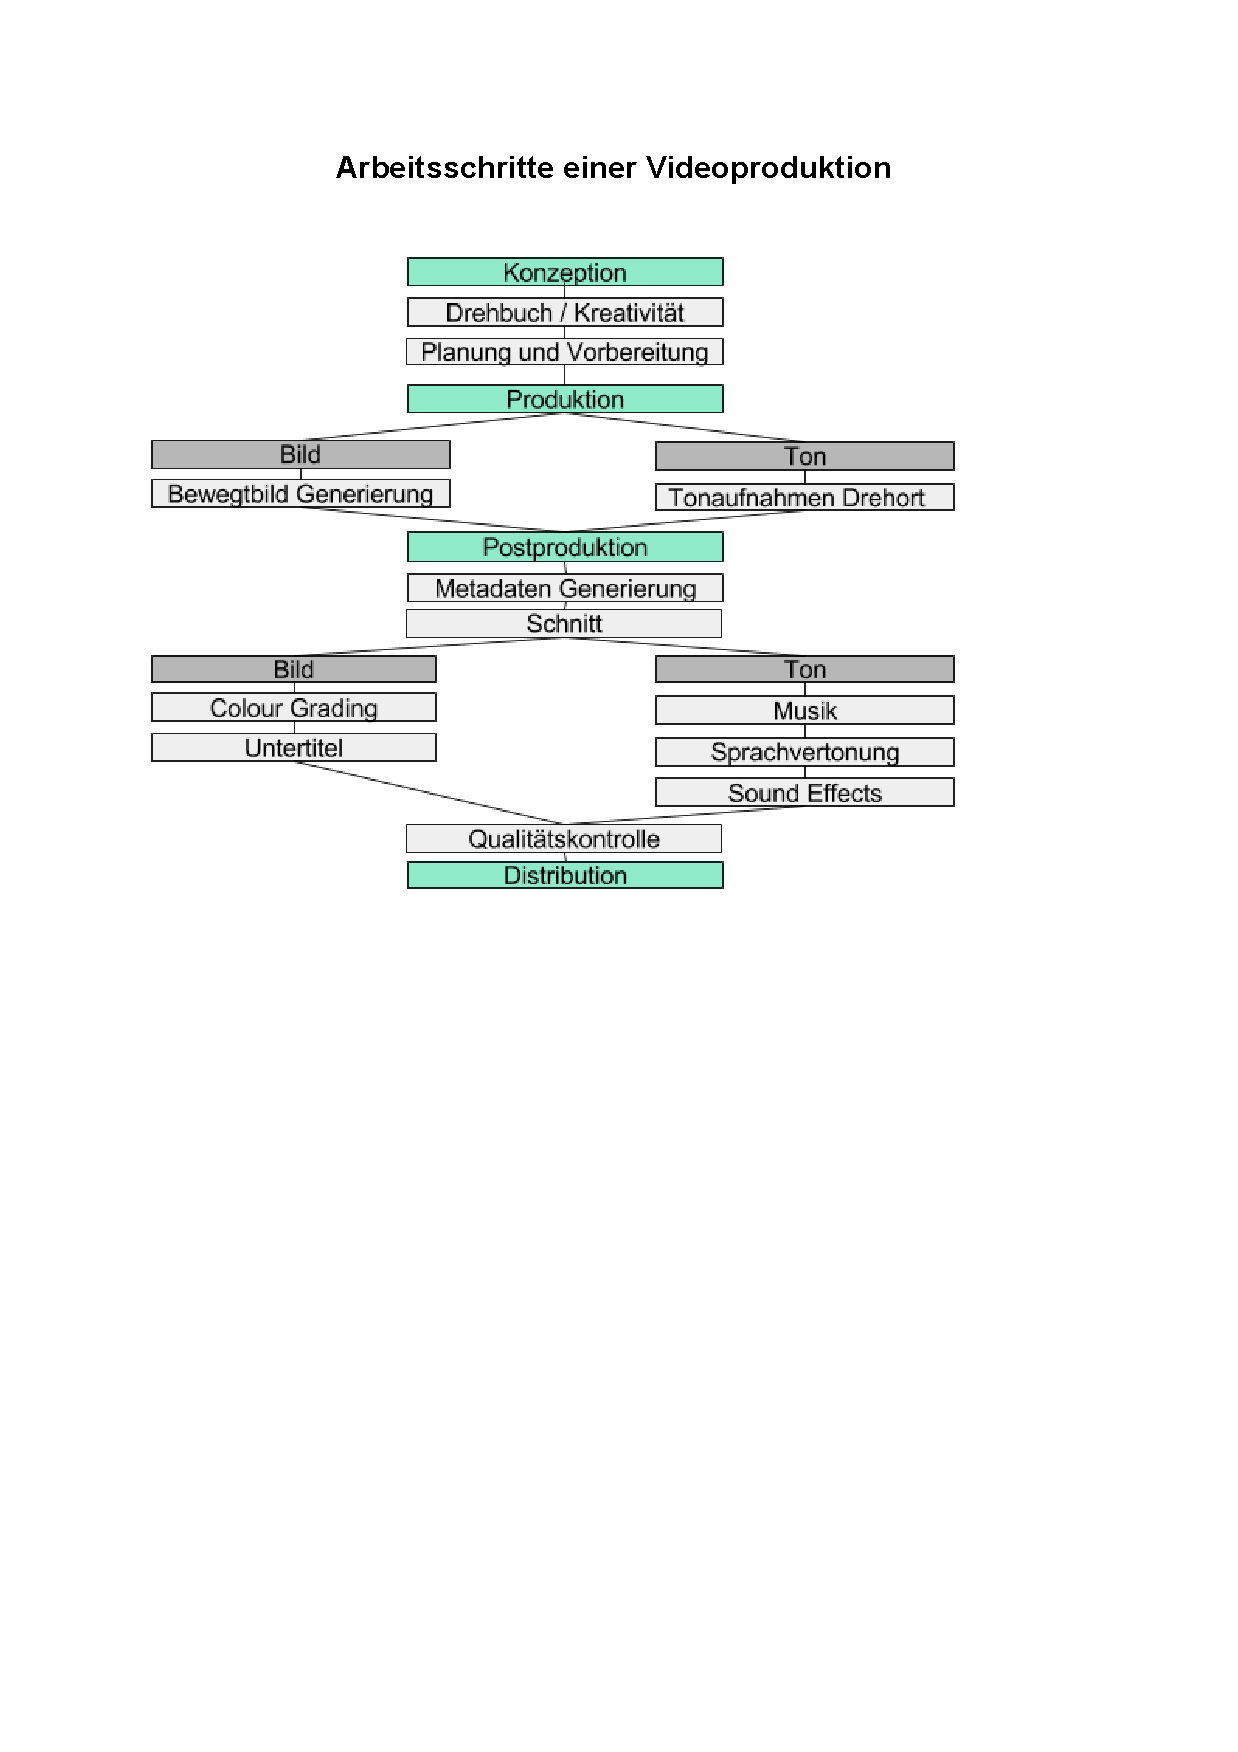
\includegraphics[width=\columnwidth, trim = 20mm 145mm 45mm 40mm, clip]{Bilder/ArbeitsschritteVideoproduktion.pdf}
	\caption{Grundlegende Arbeitsschritte einer Videoproduktion.}
	\label{fig:Videoproduktion}
\end{figure}
\SubSection{Neuronale Netze} \label{sec:NeuronaleNetze}
\todo[inline, color=yellow]{Laura} 

NNs finden unter anderem Anwendung bei der Steuerung von Robotern, Börsenkursanalysen, Medizin oder Fahrzeugsteuerung. In der Bildverarbeitung werden NNs vor allem zur Klassifizierung genutzt. \\
Sie sind vom menschlichen Gehirn inspiriert, welches laut \cite{NNHaykin} ein nicht-lineares, komplexes und hoch paralleles System zur Verarbeitung von Informationen darstellt. Ähnlich wie dieses bestehen künstliche NNs aus einer Menge an simulierten Neuronen, die untereinander verbunden sind und in Schichten organisiert sind. Es gibt verschiedene Arten der Vernetzung, die, wie in \cite{NNHaykin} und \cite{NNStanley} beschrieben, in rück- und vorwärts gekoppelte Modelle unterteilt werden können.\\

\begin{figure}
	\flushleft
	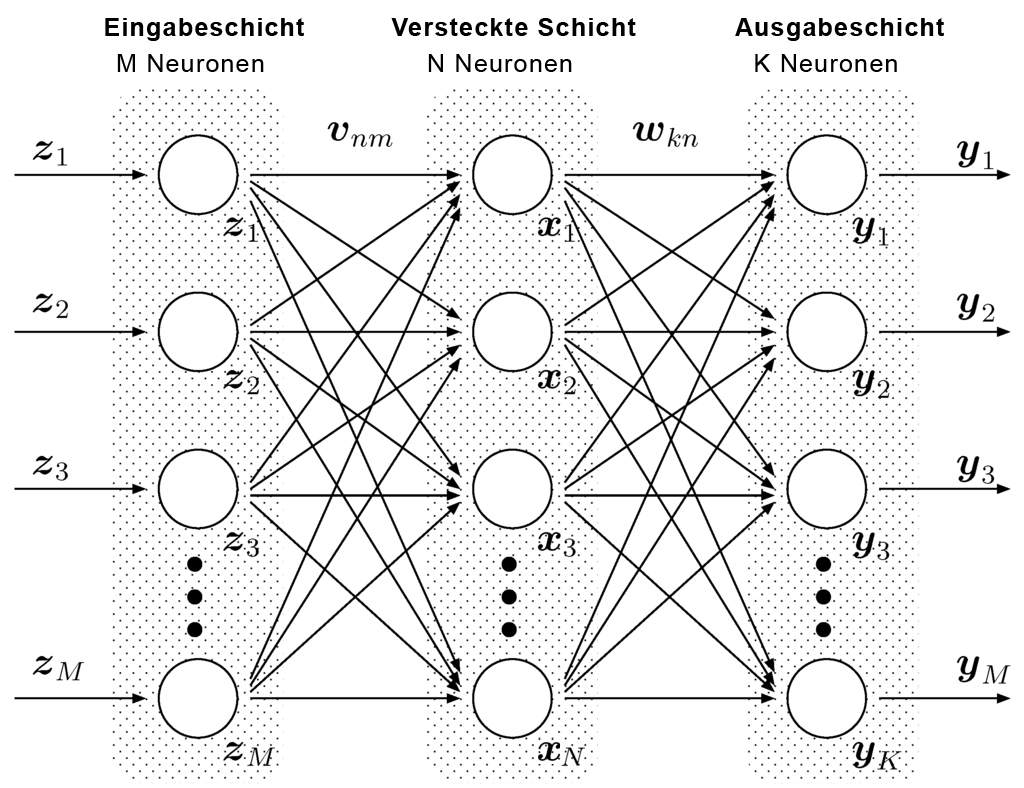
\includegraphics[width=\columnwidth]{Bilder/structure-mlp.jpg}
	\caption{Prinzipieller Aufbau MLP nach \cite{MDPI}.}
	\label{fig:MLP}
\end{figure}

Am häufigsten kommen sogenannte \textit{Multilayer Perceptrons} (MLP)  \cite{NNBraun}\cite{NNNauck}\cite{NNStanley} zum Einsatz. Wie der Name vermuten lässt, werden hierbei die Neuronen in Schichten angeordnet. Ein solcher Aufbau ist beispielhaft in Abbildung~\ref{fig:MLP} zu sehen. Dieses MLP besteht aus eine Eingabe- und Ausgabeschicht mit $M$ bzw $K$ Neuronen und einer versteckten Schicht mit $N$ Neuronen. Es handelt sich um ein vorwärtsgekoppeltes Modell, bei welchem jedes Neuron einer Schicht mit jedem Neuron der darauffolgenden Schichte verbunden ist. Dies nennt man volle Verbindung. Die Eingangsschicht dient zum Verteilen der Eingangswerte $z_m$ mit $m=1,...,M$. Die Ausgabe eines jeden Neurons in der versteckten Schicht, dargestellt durch $x_n$, lässt sich durch Formel \ref{eq:AusgabeVerdeckteSchicht} berechnen. Hierbei steht $v_{nm}$ für die jeweilige Gewichtung der Verbindungen zwischen den Neuronen der Eingabe- und der versteckten Schicht und $f$ für die Aktivierungfunktion~\cite{NNStanley}\cite{NNHaykin} des jeweiligen Neurons. 

\footnotesize
\begin{equation} 
x_n = f~(\sum_{m=1}^M v_{nm}z_m)
	\label{eq:AusgabeVerdeckteSchicht}
\end{equation}
\small

Die Ausgangswerte $y_k$, mit $k=1,...,K$, lassen sich äquivalent unter Hereinnahme der Werte $x_n$ und der Gewichte $w_{kn}$, sowie einer Aktivierungsfunktion $g$ berechnen, und gelten als Vertrauenswerte. Sie müssen gemäß der Aufgabenstellung interpretiert werden. 


\SubSection{Faltungsnetze} \label{sec:Faltungsnetze}
\todo[inline, color=red]{Laura} 
Im Folgenden wird genauer auf Faltungsnetze eingegangen, da diese die Grundlage, für die meisten der in den folgenden Kapiteln vorgestellten Ansätze, bilden. Vereinfacht ausgedrückt besteht ein Faltungsnetz aus einer Vernetzung von Faltungsoperationen mit unterschiedliche Filtermasken. Faltungsnetze kommen, bedingt durch ihre Architektur, oft zum Einsatz, wenn große Datenmengen von einem NN verarbeitet werden sollen. Ein schematischer Aufbau ist in Abbildung~\ref{fig:CNN} zu sehen. 

\begin{figure}
	\flushleft
	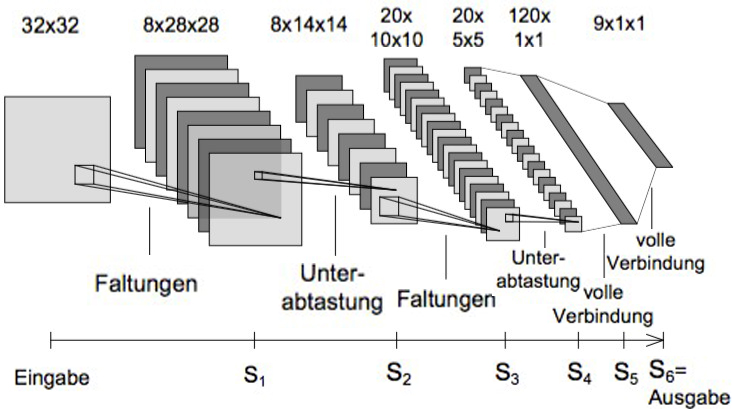
\includegraphics[width=\columnwidth]{Bilder/structure-cnn.jpg}
	\caption{Prinzipieller Aufbau Faltungsnetz nach \cite{Osadchy}.}
	\label{fig:CNN}
\end{figure}

Jedes Pixel eines Feldes, das auf der Abbildung zu sehen ist, wird durch ein Neuron repräsentiert. Die Felder sind in Schichten organisiert. Die Eingangsschicht fungiert, vergleichbar wie bei den MLPs aus Kapitel~\ref{sec:NeuronaleNetze}, als Verteiler der Information an die Neuronen der nächsten Schicht $S_1$. Die Besonderheit eines Faltungsnetzes sind die sich abwechselnd durchgeführte Faltung und anschließende Unterabtastung. Zwischen den Schichten $S_4$ und $S_6$ ähnelt das Modell einem MLP, da die Neuronen schichtweise voll verbunden sind.\\

Im Allgemeinen wird für eine Faltung eine Filtermaske $h$, also eine endlicher zweidimensionaler Koeffizientensatz, wie in Formel~\ref{eq:Filtermaske} zu sehen, verwendet. Hierbei stehen $x$ und $y$ jeweils für die horizontale bzw. die senkrechte Bildkoordinate. Die Anzahl der Koeffizienten $a_{xy}$, wird in der Horizontalen mit $N_{hx}$ und im Vertikalen mit $N_{hy}$ bezeichnet. 

\footnotesize
\begin{equation} 
	h(x,y) = \left\lbrace
  \begin{array}{l@{}l}
   0~f\ddot{u}r~x<-\lfloor\frac{N_{hx}-1}{2}\rfloor~\vee~y<-\lfloor\frac{N_{hy}-1}{2}\rfloor\\
    0~f\ddot{u}r~x>\lfloor\frac{N_{hx}-1}{2}\rfloor~~~~\vee~y>\lfloor\frac{N_{hy}-1}{2}\rfloor \\
    a_{xy}
  \end{array}
  \right.	
	\label{eq:Filtermaske}
\end{equation}
\small  

Formel~\ref{eq:Faltung} beschreibt die Faltung eines Eingangssignals $s$ mit einer Filtermaske $h$, wobei I das Ausgangssignal in Abhängigkeit von $x$ und $y$ beschreibt.

\footnotesize
\begin{equation}
\begin{aligned}
I(x,y) = (s*h)(x,y) = \\
\sum_{m_x=-\infty}^\infty \sum_{m_y=-\infty}^\infty s(m_x,m_y) \cdot h(x-m_x,y-m_y) 
\end{aligned}
	\label{eq:Faltung}
\end{equation}
\small

Im Fall eines Faltungsnetzes wird die Faltung, die wie in Abbildung~\ref{fig:CNN} zu sehen, beispielsweise zwischen der Eingangsschicht und $S_1$ vollzogen wird, wird durch die Verbindung zwischen den Neuronen zweier Felder modelliert. Dabei entsprechen die Gewichte der Neuronen genau den Filterkoeffizienten $a_{xy}$. Für ein jedes Feld sind diese Koeffizienten konstant, was bedeutet, dass alle Neuronen eines Feldes mit nur einem Gewicht auskommen. Dieses Prinzip nennt man geteilte Gewichte. \\

Im Faltungsnetz wird nach jeder Faltung eine Unterabtastung durchgeführt um zu gewährleisten, dass die Dimension der Eingangsdaten schrittweise an die Dimension des Ausgangsvektors angepasst wird. Hierzu wird meist eine bilineare Unterabtastung um den Faktor 2 vorgenommen. \\

Wie zu Beginn des Kapitels erwähnt, haben Faltungsnetze gegenüber den MLPs den Vorteil, dass sie nahezu beliebig hochskaliert werden können und somit gut geeignet für große Datenmengen sind. Dies liegt vor allem daran, dass die Neuronen nur lokal verbunden sind und sich somit das Prinzip der geteilten Gewichte zu Nutze gemacht werden kann. Ein weiterer Vorteil von Faltungsnetzen, der vor allem in der Bildverarbeitung genutzt wird, ist das sie translationsinvariant sind.


\Section{Vorverarbeitung} \label{sec:Vorverarbeitung}
\todo[inline, color=red]{Vera} 
\SubSection{Aktueller Stand} \label{sec:SOTAVorverarbeitung}
\todo[inline, color=red]{Vera} 

\Section{Produktion} \label{sec:Produktion}
\todo[inline, color=red]{Laura} 
\SubSection{Aktueller Stand} \label{sec:SOTAProduktion}
\todo[inline, color=red]{Laura} 
\SubSection{Szenendynamik nach Vondrick} \label{sec:Vondrick}
\todo[inline, color=red]{Laura} 

\Section{Postproduktion} \label{sec:Postroduktion}
\todo[inline, color=red]{Vera} 
\SubSection{Aktueller Stand} \label{sec:SOTAPostproduktion}
\todo[inline, color=red]{Vera} 

\Section{Zusammenfassung} \label{Zusammenfassung}
\todo[inline, color=red]{Vera} 





\bibliographystyle{latex8} 
\bibliography{psm.bib}

\end{document}

